\section{Docker Architecture}
\label{sec::arch}

% 3. Docker Architecture
%     1. The Docker engine
%         1. Client server
%         2. Monolithic architecture
%         3. runc
%         4. containerd
%     2. Images
%         1. Layers
%         2. Dockerfile
%         3. Docker compose
%     3. Containers
%         1. Container creation process
%         2. Workflow
%     5. Volumes and persistent data
%     6. Networking

% TODO:
% explain libcontainer

\subsection{Docker Engine}
\label{sec::arch:engine}

The Docker Engine is the core software responsible for running and managing containers, which consists of several modular components\cite{Docker-engine}. It is implemented as a client-server application, consisting of:

\begin{itemize}
    \item A server running the daemon process \texttt{dockerd};
    \item Docker's \acs{REST}ful \acs{API};
    \item The \acs{CLI} client, \texttt{docker}.
\end{itemize}

Within this architecture, the Docker daemon is the component responsible for creating, running and managing the containers. The daemon is able to manage any number of containers in the device, all controlled via the \acs{CLI} client. The client interacts with the Docker daemon via its own \acs{REST} \acs{API} over Unix sockets or a network interface\cite{Poulton2020-ju}.

\begin{figure}[!htb]
    \centering
    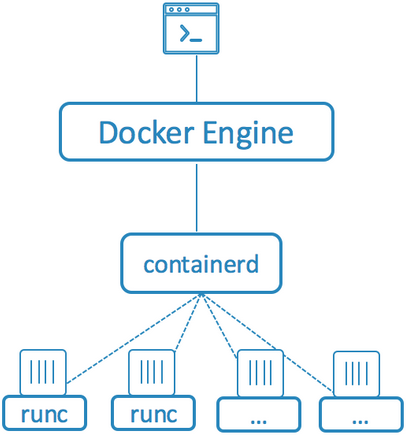
\includegraphics[width=0.25\textwidth]{docker_engine.png}
    \caption{Diagram representative of the Docker Engine architecture\cite{fig-src:docker-engine}.}
    \label{fig::docker-engine-server}
\end{figure}

Despite being, at its core, a client-server architecture, Docker's server is far from monolithic (figure \ref{fig::docker-engine-server}). The server operates a set of smaller components, among them \texttt{runc} and \texttt{containerd}, the main modules responsible for creating and running containers. Both implement as closely as possible the \ac{OCI} open source project specifications~\cite{Poulton2020-ju, oci-runc, git-runc, docker-containerd}.

The first program, \texttt{runc}, is a \acs{CLI} component responsible for creating and running applications. Its purpose is to be a standalone low-level tool called by any high-level application, such as Docker. In order to achieve this, \texttt{runc} relies on the library \texttt{libcontainer} to access the container isolation features of the \acs{OS}, such as \texttt{seccomp} and user namespaces\cite{runc-estes}.

Secondly, \texttt{containerd} is responsible for managing all the container execution logic, such as starting, stopping and removing containers. In the same way as \texttt{runc}, \texttt{containerd} is available as a standalone daemon and was intended to be a lightweight program with the sole role of managing container lifetime operations. But as it grew, it gained new functionalities, such as data storage and image management\cite{docker-containerd}.

With this in mind, it's possible to understand the container creation workflow. When a command is typed in the \acs{CLI}, the Docker client converts the instructions into the \acs{API} payload and POSTs to the correct API endpoint. Once the daemon receives the command to create a new container, a call is made to \texttt{containerd}, which converts the required Docker image into a bundle and instructs \texttt{runc} to create a new container. In its turn, \texttt{runc} interfaces with the \acs{OS} kernel to allocate the resources and to execute the instructions needed to create a new container. The container process is started as a child-process of \texttt{runc}, and as soon as it is started, \texttt{runc} is terminated.



\subsection{Containers}
\label{sec::arch:containers}

As defined by the \texttt{libcontainer} README page\cite{docker-libcontainer}:

\begin{displayquote}
    ``\textit{A container is a self-contained execution environment that shares the kernel of the host system and is optionally isolated from other containers in the system.}''
\end{displayquote}

Despite the behavior similarities between containers and \acsp{VM}, they are fundamentally different since all the containers running in the system share the same kernel, so the isolation between workloads is implemented within that one kernel. As a result, there is one less layer of abstraction between the isolated task and the hardware underneath, which results in better resource efficiency.

However, it's only possible to run processes that are compatible with the underlining kernel, \ie~ a Windows container cannot run Linux application and vice-versa.



\subsection{Images}
\label{sec::arch:images}

Docker images are a template of what is reconstructed into a running container; it serves as a base for everything that will be deployed and run on the container, similarly to a filesystem \cite{Kane2018-fn}. Before launching a container, the image must be built from scratch or downloaded from a public registry. When the \texttt{docker pull} command is used, the default registry used is the official Docker Hub \cite{docker-hub}.

An image consists of multiple read-only layers; each layer represents the changes made to the underlining system, \ie~ a \texttt{diff} of the previous layer \cite{images-layers}. When a container is created, a new read-write layer is added on top of the previous ones, so that all the changes made during the container execution are saved on disk (figure \ref{fig:docker-image}) \cite{fig-src:image-layers}.

A layer is identified by a digest, referred to as \textit{Content Addressable IDs}, as each hash represents the image content. This model of layer separation allows several images to address the same layer. As such, the latter only needs to be stored once in the device.

\begin{figure}[!htb]
    \centering
    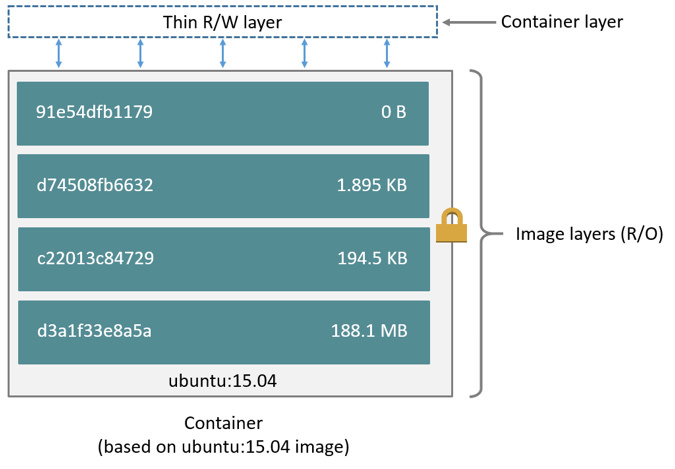
\includegraphics[width=0.45\textwidth]{container-layers.jpg}
    \caption{Diagram exemplifying a Docker image composition, where the set of layers composes an Ubuntu container \cite{fig-src:image-layers}.}
    \label{fig:docker-image}
\end{figure}

These layers are described in the image manifests, which are \acs{JSON} files containing both information about the image's layers and a list of compatible architectures given by an image tag \cite{image-manifest}.

Docker uses a storage driver to store and manage image layers. This component is also responsible for writing on the write-layer of the image. The data written by the storage driver does not persist after the container is deleted, thus being more suitable for storing data generated during application runtime\cite{storage-driver}.

For applications that require persistent storage, even when the container is deleted, or if necessary to supply other containers access to that data, it's required to create a volume.



\subsection{Volumes and persistent data}
\label{sec::arch:volumes}

When a container is created, the system automatically allocates local storage where the container's filesystem is stored. However, this integral part of the container is tied to it's lifecycle: it will be deleted as soon the container itself is deleted. By default, the container only uses such local storage. If data persistence is needed, there are two options for containers to store data on the host device: volumes and bind mounts\cite{container-storage}.

Volumes are created and managed by Docker and are stored within a folder on the host machine. As volumes are only managed by Docker, this means they are isolated from the host and only Docker is allowed to write any change made to the volume. It's possible to mount a single volume into multiple containers. When a given volume isn't being used by any container it won't be removed automatically.

On the other hand, bind mounts consist on directories on the host machine being mounted into a container. This mounts are limited in functionality as they are not managed by Docker itself.



\subsection{Networking}
\label{ssec::arch:net}

Docker containers are able to establish network connections both between one or various containers, and non-container networks. When a container is attached to a Docker network, an unique \acs{IP} address is attributed to said container. Docker networks are regarded as first-class entities, each having their own life cycle, and are not dependent on other components, being composed of three main modules\cite{Poulton2020-ju}:

\begin{itemize}
    \item \textbf{\ac{CNM}} --- the network's design specifications which outlines the fundamental building blocks of a docker network;
    \item \textbf{\texttt{libnetwork}} --- native Go implementation of the core components outlined in the \ac{CNM};
    \item \textbf{Network drivers} --- pluggable interfaces that provide the networking subsystem.
\end{itemize}

To fully comprehend the different network configurations available, it's important the underlining building blocks of the \ac{CNM} interface. Each container defines a \textbf{network sandbox}, which is an isolated environment containing the networking configuration of the container, including Ethernet interfaces, ports, routing tables and \acs{DNS} configuration. A network sandbox may contain multiple \textbf{endpoints}, \ie~the virtual network interfaces responsible for maintaining the connection between the sandbox and a given network. A \textbf{network} is a uniquely identifiable group of endpoints capable of communicating with each other, connecting different networking sandboxes.

\begin{figure}[!htb]
    \centering
    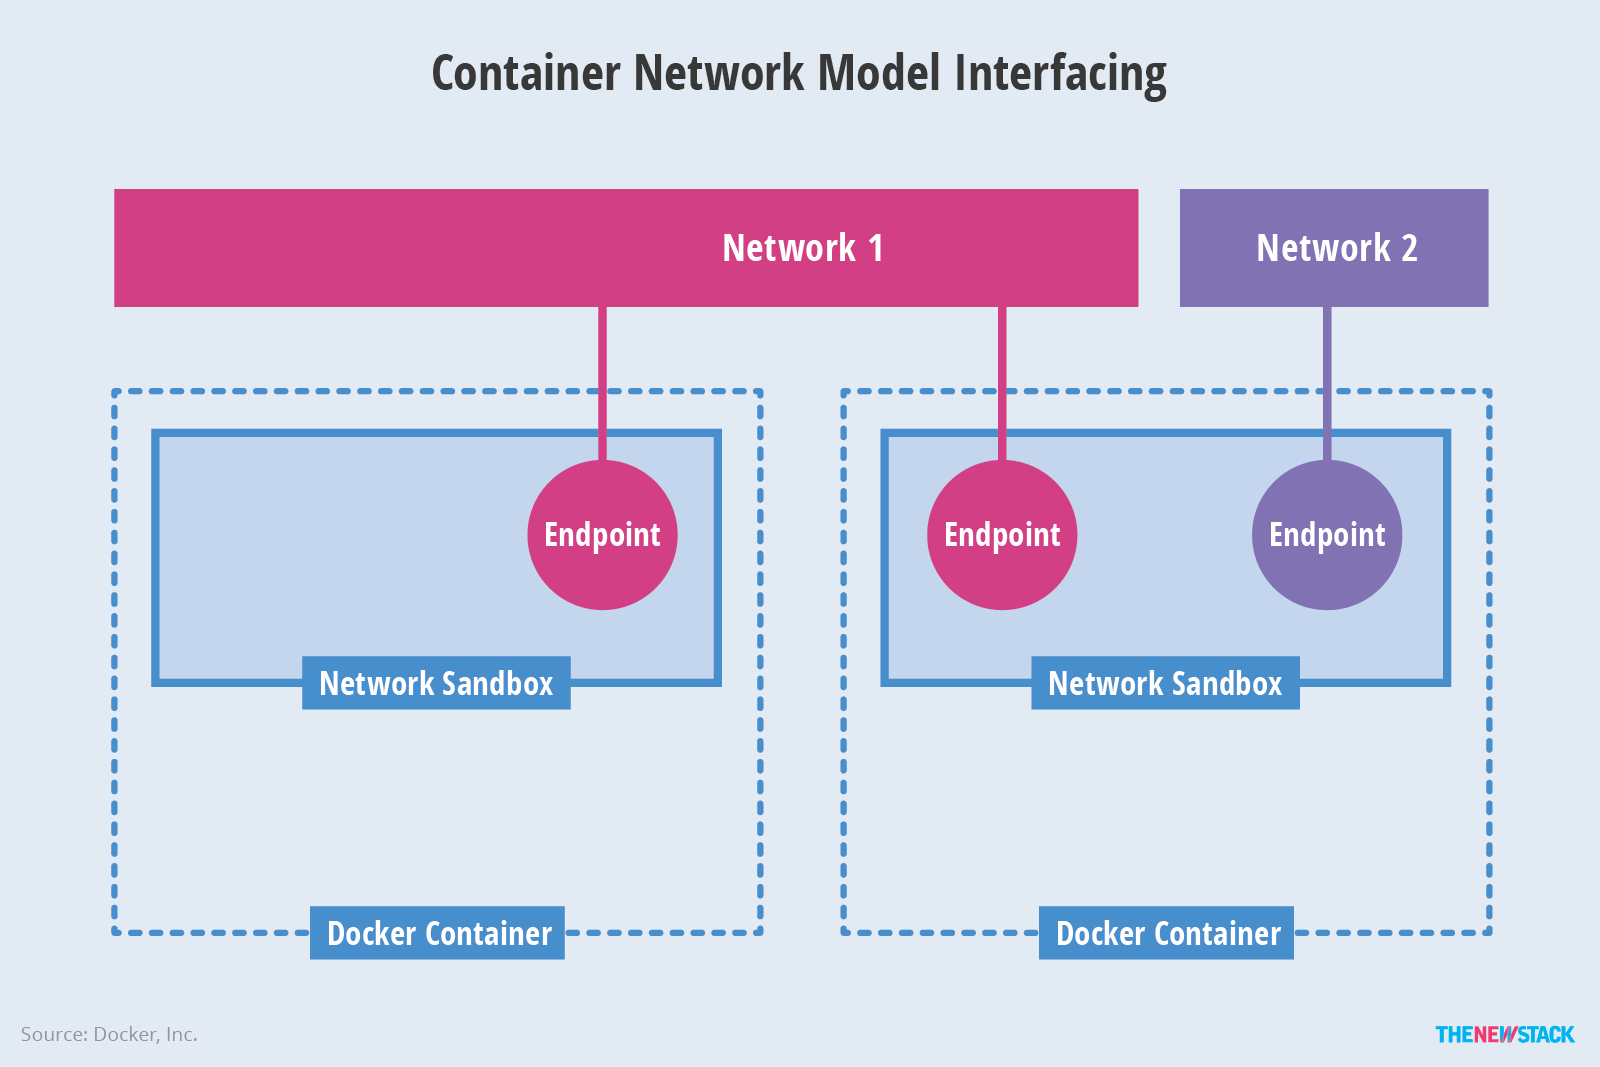
\includegraphics[width=0.45\textwidth]{cnm-interface.png}
    \caption{Diagram representing the architecture of \ac{CNM} \cite{fig-src:cnm}.}
    \label{fig:cnm-interface}
\end{figure}

Based on these building blocks, the \texttt{libnetwork} is the core implementation of the networking functionalities defined by the \ac{CNM}. The drivers are responsible for handling the connectivity and isolation of the network objects (figure \ref{fig:cnm-drivers}).

\begin{figure}[!htb]
    \centering
    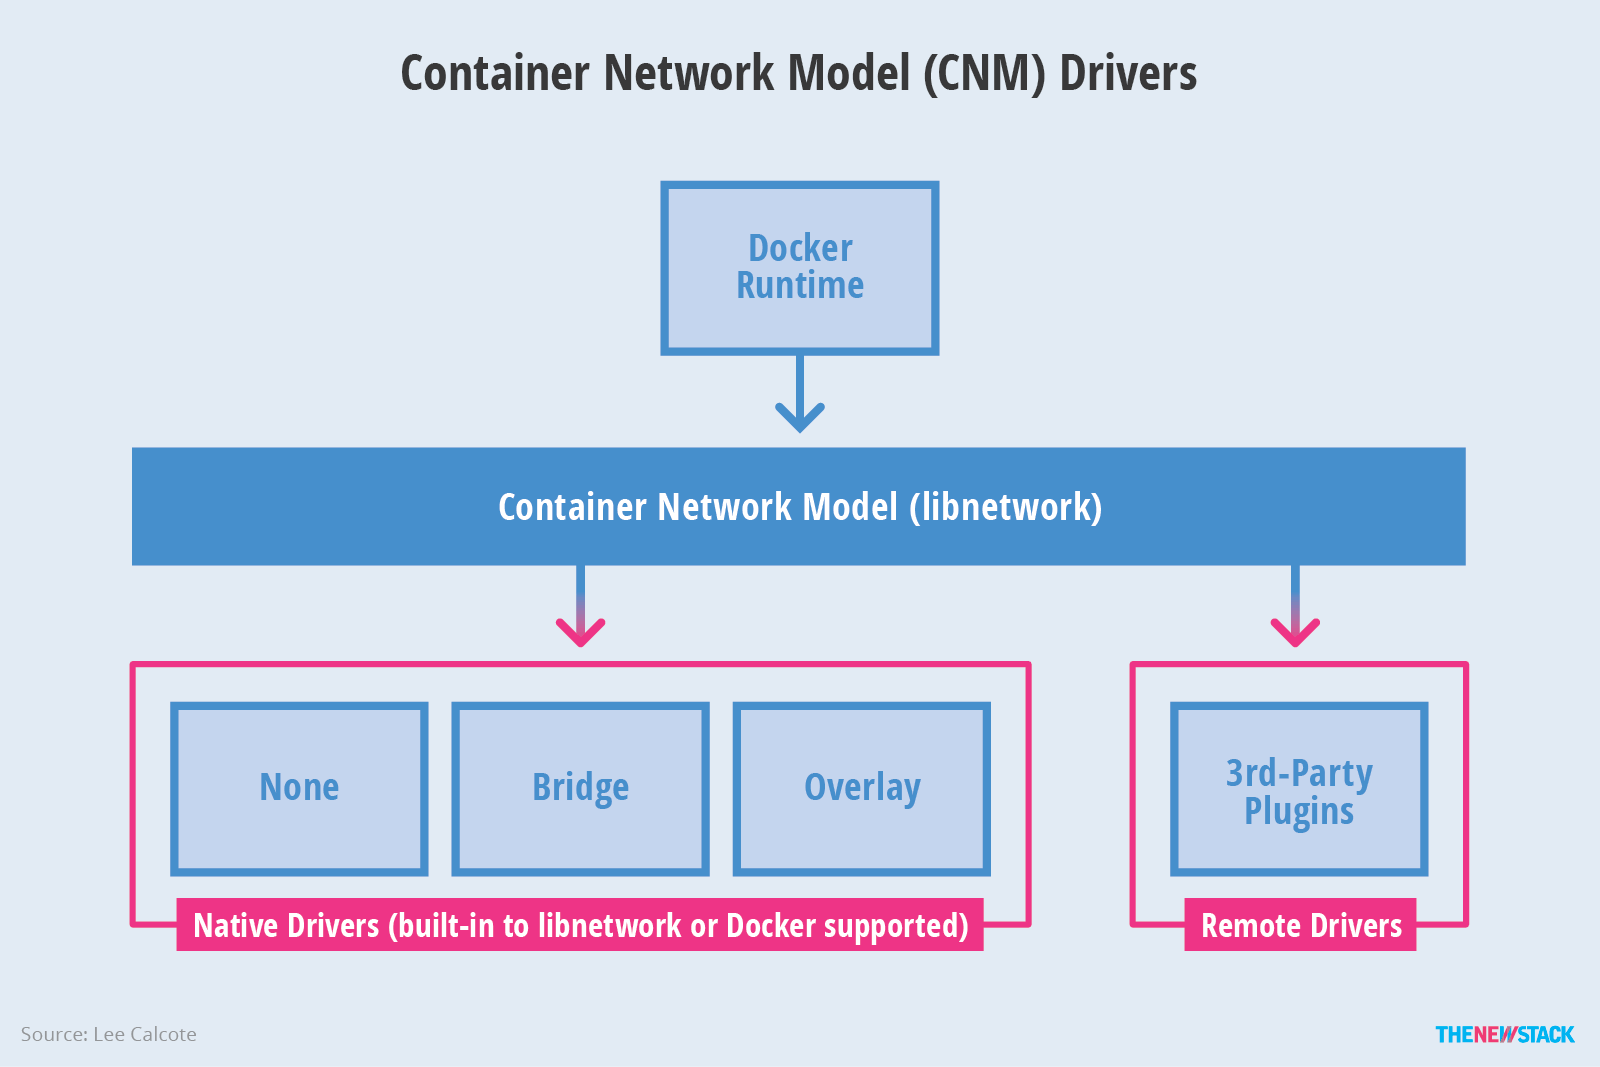
\includegraphics[width=0.45\textwidth]{cnm-drivers.png}
    \caption{Diagram demonstrating how the Docker deamon interacts with the various drivers via the \texttt{libnetwork} \cite{fig-src:cnm}.}
    \label{fig:cnm-drivers}
\end{figure}

It's possible to implement and use 3rd-party drivers, but Docker is shipped with several built-in drivers, known as native or local drivers\cite{network-drivers}. These include:

\begin{itemize}
    \item \texttt{bridge} --- provides an implementation of a 802.1d bridge (layer 2 switch) between containers running on the same machine. The default bridge network maps to an underlying Linux bridge in the host's kernel named ``\texttt{docker0}'', which is in its turn mapped back to an Ethernet interface on the host via port mappings\cite{network-bridge};
    
    \item \texttt{host} --- the container's network stack is not isolated from Docker's host. This driver instructs Docker not to create any networking namespace or resource for attached containers. Containers on this network will interact with the host's network just like uncontained processes. Despite this, all the other aspects of the container will be isolated \cite{network-host};
    
    \item \texttt{overlay} --- connects Docker daemons running on different hosts; widely used on swarm services \cite{network-overlay};
    
    \item \texttt{macvlan} --- allows to attach a \acs{MAC} address to a container, making it appear as a physical device on the network\cite{network-mac};
    
    \item \texttt{ipvlan} ---gives the user complete control over IPv4 and IPv6 addressing\cite{network-ipvlan};
    
    \item \texttt{none} --- uses the null driver, meaning the containers attached to the network won't have any network connection outside themselves.
\end{itemize}

These configurations fall under three categories: local, global or swarm. It indicates whether the network is constrained to the machine where the network exists (local), should be created on every node in a cluster but not route between them (global), or seamlessly spans all of the hosts participating in a Docker swarm (multi-host or cluster-wide)\cite{Poulton2020-ju}. The default networks have a local scope, and will not be able to directly route traffic between containers running on different machines\cite{network-drivers}.